% ============================================================
%  Multi-Signature Treasury for Student Clubs
%  CSCI 435 — Blockchain Engineering
%  Final Project Report
% ============================================================
\documentclass[12pt,a4paper]{article}

\usepackage[margin=2.5cm]{geometry}
\usepackage{graphicx}
\usepackage{hyperref}
\usepackage{xcolor}
\usepackage{listings}
\usepackage{booktabs}
\usepackage{enumitem}
\usepackage{fancyhdr}
\usepackage{titlesec}
\usepackage{amsmath}
\usepackage{parskip}
\usepackage{array}
\usepackage{tabularx}
\usepackage{longtable}
\usepackage{multirow}
\usepackage{mdframed}
\usepackage{tikz}
\usetikzlibrary{shapes.geometric, arrows.meta, positioning, fit}

% ── Hyperlinks ────────────────────────────────────────────
\hypersetup{
  colorlinks=true, linkcolor=blue!70!black,
  urlcolor=blue!70!black, citecolor=blue!70!black
}

% ── Solidity code style ───────────────────────────────────
\definecolor{codebg}{HTML}{1e293b}
\definecolor{codecomment}{HTML}{6a9955}
\definecolor{codekeyword}{HTML}{569cd6}
\definecolor{codestring}{HTML}{ce9178}
\definecolor{codenumber}{HTML}{b5cea8}

\lstdefinelanguage{Solidity}{
  keywords={pragma, solidity, contract, function, returns, external, public,
            internal, view, pure, payable, memory, storage, calldata,
            mapping, address, uint256, bool, string, bytes, struct, event,
            emit, require, modifier, if, else, for, while, return,
            constructor, true, false, uint, bytes32, indexed, receive},
  comment=[l]{//},
  morecomment=[s]{/*}{*/},
  string=[b]",  morestring=[b]',  sensitive=true
}

\lstset{
  language=Solidity,
  backgroundcolor=\color{codebg},
  basicstyle=\ttfamily\small\color{white},
  keywordstyle=\color{codekeyword}\bfseries,
  commentstyle=\color{codecomment}\itshape,
  stringstyle=\color{codestring},
  numberstyle=\tiny\color{codenumber},
  numbers=left, numbersep=8pt,
  breaklines=true, frame=single, framesep=4pt,
  rulecolor=\color{gray!40}, tabsize=4,
  showstringspaces=false, captionpos=b
}

% ── Header / footer ───────────────────────────────────────
\pagestyle{fancy}
\fancyhf{}
\lhead{\small Multi-Signature Treasury for Student Clubs}
\rhead{\small CSCI 435 — Blockchain}
\cfoot{\thepage}

% ── Section formatting ────────────────────────────────────
\titleformat{\section}{\large\bfseries\color{blue!70!black}}{\thesection.}{0.5em}{}[\titlerule]
\titleformat{\subsection}{\normalsize\bfseries}{\thesubsection}{0.5em}{}

% ─────────────────────────────────────────────────────────
\begin{document}

% ══════════════════════════════════════════════════════════
%  Title page
% ══════════════════════════════════════════════════════════
\begin{titlepage}
  \centering
  \vspace*{1.5cm}
  {\Huge\bfseries Multi-Signature Treasury\\[0.4em]
   for Student Clubs\par}
  \vspace{0.8cm}
  {\large\itshape Decentralised Financial Governance on Ethereum\par}
  \vspace{1.8cm}
  {\large
    \begin{tabular}{ll}
      \textbf{Name} & \textbf{Student ID} \\[4pt]
      Akhmed Assentay & 201842715 \\
    \end{tabular}
  }
  \vspace{1.2cm}
  {\large
    Course: CSCI 435 — Blockchain Engineering \\[0.3em]
    Department of Computer Science \\[0.3em]
    Submission Date: \today
  }
  \vfill
  \begin{mdframed}[backgroundcolor=gray!10, linecolor=blue!40, linewidth=1pt,
                   innerleftmargin=12pt, innerrightmargin=12pt,
                   innertopmargin=8pt, innerbottommargin=8pt]
    \centering\itshape
    ``Any transaction of club funds requires agreement from\\
    at least 2 out of 3 elected executives.''
  \end{mdframed}
\end{titlepage}

\tableofcontents
\newpage

% ══════════════════════════════════════════════════════════
\section{Introduction}
% ══════════════════════════════════════════════════════════

\subsection{Problem Statement}

Student clubs routinely raise membership fees, solicit donations and use this money on activities, equipment and travel. Traditional clubs place financial control into the hands of a single treasurer- one point of failure. Money may also be wasted in the event that the treasurer is not available, behaves independently, misplaces his or her credentials or the organization loses the treasurer.
\subsection{Why This Problem Matters}

\begin{itemize}
  \item A single treasurer is able to empty the treasury at will without checks.
  \item No clear audit trail- members do not have the ability to independently check spending.
  \item The loss or change of leaders may paralyze club funds in case of key change or loss.
  \item Budgetary disputes lack a mechanism of being resolved on-chain.
\end{itemize}

\subsection{What the Project Solves}

This project implements a \textbf{Multi-Signature (Multi-Sig) Treasury} Treasury smart contract to ensure that any transaction going out is approved by \textbf{2 out of 3} elected club executives. No individual can transfer funds independently and all offers, consent and actions are forever etched on the Ethereum blockchain.
\subsection{Blockchain Solution Overview}

The system is composed of three layers:
\begin{enumerate}
  \item A \textbf{Solidity smart contract} deployed on Ethereum (Hardhat local / Sepolia testnet).
  \item A \textbf{Hardhat} development environment with a comprehensive test suite (75 tests).
  \item A \textbf{browser DApp} (HTML + ethers.js v6) connected to wallets via MetaMask.
\end{enumerate}

% ══════════════════════════════════════════════════════════
\section{Project Objectives}
% ══════════════════════════════════════════════════════════

\subsection{Main Objectives}

\begin{enumerate}
  \item Implement a trustless 2-of-3 multi-sig spending mechanism for a student club treasury.
  \item Ensure every executive's vote is meaningful from the moment they propose a transaction.
  \item Support on-chain governance for leadership transitions (executive address replacement).
  \item Provide an emergency pause mechanism to freeze spending during a security incident.
  \item Enforce per-category spending budgets to prevent overspending in any one area.
  \item Maintain a transparent donor leaderboard on-chain.
\end{enumerate}

\subsection{Expected Functionality}

\begin{itemize}
  \item Any executive can propose, approve, revoke, or execute spending transactions.
  \item A new address replaces an executive wallet without redeploying the contract.
  \item Stale proposals (older than 7 days) can be cancelled by any executive.
  \item Anyone can deposit ETH; only executives can withdraw through the approval process.
  \item The DApp reflects real-time contract state and supports all contract functions.
\end{itemize}

\subsection{Target Users}

\begin{itemize}
  \item \textbf{Club executives} (President, Vice-President, Treasurer) — manage funds.
  \item \textbf{Club members and guests} — donate ETH and audit spending history.
\end{itemize}

% ══════════════════════════════════════════════════════════
\section{System Overview}
% ══════════════════════════════════════════════════════════

\subsection{Components of the System}

\begin{table}[h]
  \centering
  \begin{tabularx}{\linewidth}{>{\bfseries}lX}
    \toprule
    Component & Description \\
    \midrule
    \texttt{MultiSigTreasury.sol} & Core Solidity smart contract. Stores all state and enforces governance rules on-chain. \\
    Hardhat & Development framework for compiling, testing, and deploying the contract. \\
    \texttt{test/MultiSigTreasury.test.js} & 75 automated tests covering all features and edge cases. \\
    \texttt{scripts/deploy.js} & Deployment script for Hardhat local and Sepolia networks. \\
    \texttt{frontend/index.html} & Single-page DApp using ethers.js v6 and MetaMask. \\
    MetaMask & Browser wallet that signs and submits transactions. \\
    Ethereum Sepolia & Public testnet for live demonstration. \\
    \bottomrule
  \end{tabularx}
  \caption{System components and descriptions}
\end{table}

\subsection{Technologies Used}

\begin{itemize}
  \item \textbf{Solidity \textasciicircum 0.8.20} - smart contract language.
  \item \textbf{Hardhat v2.22} - Ethereum development environment.
  \item \textbf{Chai} - assertion library for JavaScript tests.
  \item \textbf{ethers.js v6} - Ethereum library for the browser DApp.
  \item \textbf{HTML5 / CSS3 / Vanilla JS} - frontend (no framework dependency).
  \item \textbf{Node.js / npm} — toolchain.
\end{itemize}

\subsection{How Users Interact with the System}

In browser, executives and members open \texttt{frontend/index.html} and connect MetaMask (configured to the local Hardhat network or Sepolia) and use the UI. Each button press causes an Ethereum transaction to be signed, and mined by Hardhat or Sepolia permanently.

\subsection{Architecture Diagram}

\begin{figure}[h]
  \centering
  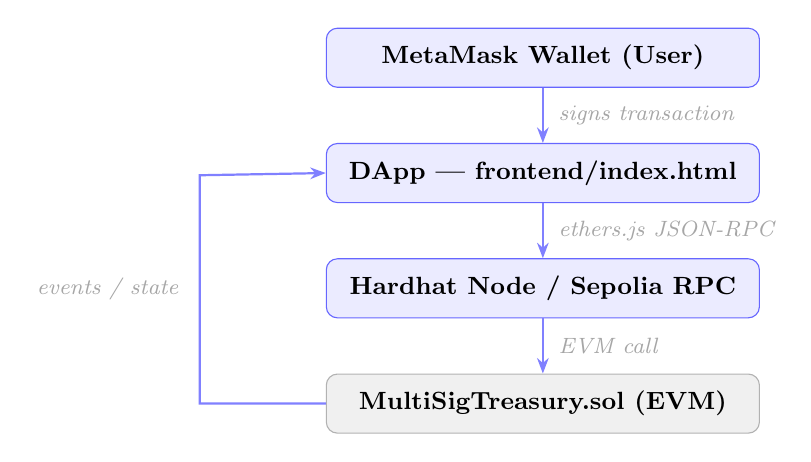
\begin{tikzpicture}[
    node distance=0.7cm,
    box/.style={rectangle, draw=blue!60, fill=blue!8, rounded corners=4pt,
                minimum width=5.5cm, minimum height=0.75cm,
                font=\small\bfseries, align=center},
    chain/.style={rectangle, draw=gray!60, fill=gray!12, rounded corners=4pt,
                  minimum width=5.5cm, minimum height=0.75cm,
                  font=\small\bfseries, align=center},
    arr/.style={-{Stealth[scale=0.85]}, thick, blue!50},
    lbl/.style={font=\footnotesize\itshape, text=gray!70}
  ]
    \node[box]   (mm)  {MetaMask Wallet (User)};
    \node[box,   below=of mm]  (ui)  {DApp — frontend/index.html};
    \node[box,   below=of ui]  (rpc) {Hardhat Node / Sepolia RPC};
    \node[chain, below=of rpc] (sc)  {MultiSigTreasury.sol (EVM)};

    \draw[arr] (mm)  -- (ui)  node[midway, right=2pt, lbl] {signs transaction};
    \draw[arr] (ui)  -- (rpc) node[midway, right=2pt, lbl] {ethers.js JSON-RPC};
    \draw[arr] (rpc) -- (sc)  node[midway, right=2pt, lbl] {EVM call};
    \draw[arr] (sc.west) -- ++(-1.6,0)
      -- ++(0,2.9) node[midway, left=4pt, lbl] {events / state}
      -- (ui.west);
  \end{tikzpicture}
  \caption{System Architecture — browser to on-chain contract}
\end{figure}

% ══════════════════════════════════════════════════════════
\section{Project Workflow}
% ══════════════════════════════════════════════════════════

\subsection{Planning Process}

\begin{enumerate}
  \item Read through the project description: 2-of-3 multi-sig treasury student club (DAO version).
  \item Found the central issue: single-treasurer risk and absence of transparency on-chain.
  \item Clarified the model of governance: propose and approve and execute lifecycle.
  \item Selected other features to earn the full marks: budget limits, emergency stop, donor leaderboard, executive change.
  \item Chosen technology stack: Solidity, Hardhat, ethers.js v6, MetaMask.
\end{enumerate}

\subsection{Development Stages}

\begin{enumerate}
  \item \textbf{Core contract} — constructor, modifiers, deposit, basic multi-sig (propose / approve / revoke / execute).
  \item \textbf{Proposer auto-approval} — had corrected the problem that the number of agreements of the proposer himself was not counted.
  \item \textbf{Spending categories} — added \texttt{category} field to proposals.
  \item \textbf{7-day expiry} — \texttt{createdAt} timestamp and \texttt{cancelExpiredTransaction()}.
  \item \textbf{Executive replacement} — independent flow of key-rotation.
  \item \textbf{Emergency pause} — 2-of-3 vote circuit breaker with reset-on-unpause.
  \item \textbf{Category budget caps} — per-category ETH cap enforced at propose and execute time.
  \item \textbf{Donor leaderboard} — \texttt{totalDonated} mapping and \texttt{\_donors} array.
  \item \textbf{Frontend DApp} — complete interface to all contract features, countdown exiry, category badge.
  \item \textbf{Test suite} —  75 automated tests in all the features and edge cases.
  \item \textbf{Documentation} — this report and LaTeX source code.
\end{enumerate}

\subsection{Testing and Debugging}

Tests were penned in parallel on each feature with Hardhat in-process network. The evm of time dependent tests (expiry) used \texttt{evm\_increaseTime} to represent passage over 7 days without waiting. The single bug detected was a category-cap assertion at the misplaced call site (propose vs. \ execute) - repaired after determining the real revert location by looking at the Hardhat stack trace.

% ══════════════════════════════════════════════════════════
\section{Smart Contract Design}
% ══════════════════════════════════════════════════════════

\subsection{Purpose of the Smart Contract}

\texttt{MultiSigTreasury} is a trustless governance contract: it stores ETH on behalf of a student club, and requires 2 of 3 people to approve each outgoing payment. It additionally manages executive identity (replacement), emergency safety (pause), budget discipline (category caps), and community transparency (donor leaderboard).

\subsection{Contract Structure}
\label{sec:contract-structure}

\subsubsection*{Constants}

\begin{lstlisting}[caption={Constants}]
uint256 public constant REQUIRED_APPROVALS = 2;
uint256 public constant MAX_EXECUTIVES     = 3;
uint256 public constant EXPIRY_PERIOD      = 7 days;
\end{lstlisting}

\subsubsection*{State Variables}

\begin{table}[h]
  \centering
  \begin{tabularx}{\linewidth}{>{\ttfamily}lX}
    \toprule
    Variable & Purpose \\
    \midrule
    executives[] & Array of 3 executive wallet addresses. \\
    isExecutive\{addr\} & O(1) lookup: is this address an executive? \\
    paused & Emergency pause flag. \\
    pauseVoteCount / unpauseVoteCount & Vote tallies for pause/unpause. \\
    hasPauseVoted\{\} / hasUnpauseVoted\{\} & Prevent double-voting on pause. \\
    transactions[] & All spending proposals (pending/executed/cancelled). \\
    hasApproved\{txIdx\}\{addr\} & Per-proposal, per-executive approval flag. \\
    categoryBudget\{key\} & Spending cap (wei) per category hash. \\
    categorySpent\{key\} & Cumulative amount spent per category. \\
    replacements[] & Executive replacement proposals. \\
    replacementApprovals\{replIdx\}\{addr\} & Approval state for replacements. \\
    totalDonated\{addr\} & Cumulative ETH donated per address. \\
    \_donors[] & Ordered list of unique donor addresses. \\
    \bottomrule
  \end{tabularx}
  \caption{Contract state variables}
\end{table}

\subsubsection*{Structs}

\begin{lstlisting}[caption={Transaction and ExecReplacement structs}]
struct Transaction {
    address to;
    uint256 value;
    string  description;
    string  category;       // e.g. "Supplies", "Events", "Equipment"
    bool    executed;
    bool    cancelled;
    uint256 approvalCount;
    uint256 createdAt;      // block.timestamp at proposal time
}

struct ExecReplacement {
    address oldExec;
    address newExec;
    uint256 approvalCount;
    bool    executed;
}
\end{lstlisting}

\subsubsection*{Events}

\begin{table}[h]
  \centering
  \begin{tabularx}{\linewidth}{>{\ttfamily}lX}
    \toprule
    Event & Emitted when \\
    \midrule
    Deposited & ETH received via \texttt{receive()} or \texttt{deposit()}. \\
    TransactionProposed & A new spending proposal is created. \\
    TransactionApproved & An executive approves a proposal. \\
    ApprovalRevoked & An executive revokes their approval. \\
    TransactionExecuted & Funds are sent to the recipient. \\
    TransactionCancelled & An expired proposal is cancelled. \\
    BudgetSet & A category spending cap is set or updated. \\
    PauseVoteCast / ContractPaused & Pause vote cast / quorum reached. \\
    UnpauseVoteCast / ContractUnpaused & Unpause vote cast / quorum reached. \\
    ReplacementProposed / Approved & Executive swap proposed / seconded. \\
    ExecutiveReplaced & Executive address swap executed on-chain. \\
    \bottomrule
  \end{tabularx}
  \caption{Contract events}
\end{table}

\subsubsection*{Modifiers}

\begin{lstlisting}[caption={Key modifiers}]
modifier onlyExecutive()  { require(isExecutive[msg.sender], "Not an executive"); _; }
modifier whenNotPaused()  { require(!paused, "Contract is paused"); _; }
modifier txExists(uint256 _i)   { require(_i < transactions.length, ...); _; }
modifier notExecuted(uint256 _i){ require(!transactions[_i].executed, ...); _; }
modifier notCancelled(uint256 _i){ require(!transactions[_i].cancelled, ...); _; }
\end{lstlisting}

\subsection{Key Functions}
\label{sec:key-functions}

\subsubsection*{5.2.1\ \ deposit() / receive()}

Accepts ETH from any address. Calls \texttt{\_recordDonation()} to track the sender in the leaderboard. Emits \texttt{Deposited}.

\subsubsection*{5.2.2\ \ proposeTransaction()}

\begin{lstlisting}[caption={proposeTransaction — core multi-sig entry point}]
function proposeTransaction(
    address _to, uint256 _value,
    string calldata _description, string calldata _category
) external onlyExecutive whenNotPaused returns (uint256 txIndex) {
    require(_to != address(0), "Invalid recipient");
    require(_value > 0, "Value must be > 0");
    require(_value <= address(this).balance, "Insufficient treasury balance");

    // Category budget check
    bytes32 key = _categoryKey(_category);
    if (categoryBudget[key] > 0)
        require(categorySpent[key] + _value <= categoryBudget[key],
                "Category budget exceeded");

    txIndex = transactions.length;
    transactions.push(Transaction({
        ..., approvalCount: 1, createdAt: block.timestamp
    }));
    hasApproved[txIndex][msg.sender] = true; // proposer auto-approved
    emit TransactionProposed(...);
}
\end{lstlisting}

The proposer's vote is recorded immediately (\texttt{approvalCount = 1}) so that every executive's agreement counts — only one additional approval is needed to reach quorum.

\subsubsection*{5.2.3\ \ approveTransaction() / revokeApproval()}

Executives who did not propose may call \texttt{approveTransaction()} to add their vote. \texttt{revokeApproval()} removes a previously cast vote. Both are blocked while the contract is paused.

\subsubsection*{5.2.4\ \ executeTransaction()}

Transfers ETH to the recipient once \texttt{approvalCount >= 2}. Sets \texttt{executed = true} \emph{before} the \texttt{call\{\}} to prevent re-entrancy. Increments \texttt{categorySpent}.

\subsubsection*{5.2.5\ \ cancelExpiredTransaction()}

Any executive may cancel a proposal that has not been executed within 7 days. This prevents stale proposals from accumulating and releases budget headroom.

\subsubsection*{5.2.6\ \ votePause() / voteUnpause()}

A pause vote can be cast by any executive. When 2 votes are cast the contract sends \texttt{paused = true}, preventing all spending functions. Unpause needs 2 additional votes and clears all the vote state to start the cycle again.
\subsubsection*{5.2.7\ \ setCategoryBudget()}

Sets a maximum cumulative ETH cap for a named category (hashed to \texttt{bytes32} key). A cap of 0 removes the limit.

\subsubsection*{5.2.8\ \ proposeReplacement() / approveReplacement() / executeReplacement()}

Mirrors the spending multi-sig but for executive roster changes. Proposer is auto-approved; one more approval triggers the swap in \texttt{executives[]} and \texttt{isExecutive}.

% ══════════════════════════════════════════════════════════
\section{Implementation Details}
% ══════════════════════════════════════════════════════════

\subsection{Programming Languages and Frameworks}

\begin{table}[h]
  \centering
  \begin{tabularx}{\linewidth}{>{\bfseries}lX}
    \toprule
    Language / Tool & Role \\
    \midrule
    Solidity 0.8.20 & Smart contract. \\
    JavaScript (CommonJS) & Hardhat config, deployment scripts, test suite. \\
    HTML5 / CSS3 / JS (browser) & Frontend DApp. \\
    Hardhat v2.22 & Compile, test, deploy. \\
    Chai & Test assertions. \\
    ethers.js v6 & JavaScript $\leftrightarrow$ Ethereum bridge (DApp \& tests). \\
    Node.js 20 / npm & Package manager and runtime. \\
    \bottomrule
  \end{tabularx}
  \caption{Technology stack}
\end{table}

\subsection{Security Implementation}

\begin{table}[h]
  \centering
  \begin{tabularx}{\linewidth}{>{\bfseries}lX}
    \toprule
    Measure & How it is implemented \\
    \midrule
    Re-entrancy guard & \texttt{txn.executed = true} is set before \texttt{call\{\}}, making a re-entrant callback revert on the \texttt{notExecuted} modifier. \\
    Access control & \texttt{onlyExecutive} modifier on every governance function. \\
    Double-vote prevention & \texttt{hasApproved}, \texttt{hasPauseVoted}, \texttt{hasUnpauseVoted} mappings enforce one vote per executive per action. \\
    Zero-address validation & Constructor and replacement proposals reject \texttt{address(0)}. \\
    Duplicate executive check & Constructor iterates and rejects duplicates before adding. \\
    Balance checks & Both propose and execute verify sufficient treasury balance. \\
    Budget enforcement & Category cap checked at propose time (early rejection) and at execute time (race-condition safety). \\
    Expiry & \texttt{notCancelled} modifier blocks interaction with cancelled proposals. \\
    Pause state & \texttt{whenNotPaused} modifier on propose, approve, and execute. \\
    \bottomrule
  \end{tabularx}
  \caption{Security measures}
\end{table}

% ══════════════════════════════════════════════════════════
\section{Project Results}
% ══════════════════════════════════════════════════════════

\subsection{Test Suite Results}

All \textbf{75 tests pass} with a total runtime of approximately 1 second on the in-process Hardhat network.

\begin{table}[h]
  \centering
  \begin{tabular}{lr}
    \toprule
    Test Group & Tests \\
    \midrule
    Deployment                  & 5  \\
    Deposits \& Donor Leaderboard & 7  \\
    Emergency Pause             & 11 \\
    Category Budget Caps        & 8  \\
    Propose Transaction         & 5  \\
    Approve Transaction         & 5  \\
    Revoke Approval             & 3  \\
    Execute Transaction         & 7  \\
    Transaction Expiry          & 5  \\
    Executive Replacement       & 6  \\
    Executive Aliases           & 7  \\
    End-to-End Scenarios        & 5  \\
    \midrule
    \textbf{Total}              & \textbf{75} \\
    \bottomrule
  \end{tabular}
  \caption{Test suite breakdown — all 75 passing}
\end{table}

\subsection{Contract Metrics}

\begin{table}[h]
  \centering
  \begin{tabular}{lr}
    \toprule
    Metric & Value \\
    \midrule
    Lines of Solidity code    & 310 \\
    Public / external functions & 18 \\
    Events defined            & 11 \\
    Modifiers defined         & 5  \\
    Structs defined           & 2  \\
    Required approvals        & 2 of 3 \\
    Expiry period             & 7 days \\
    Solidity compiler version & 0.8.20 \\
    \bottomrule
  \end{tabular}
  \caption{Contract metrics}
\end{table}

\subsection{DApp UI — Working Screenshots Description}

The browser DApp displays the following panels when MetaMask is connected:

\begin{itemize}
  \item \textbf{Status bar}: treasury balance in ETH, total proposal count, connected user role (Executive / Viewer).
  \item \textbf{Executives panel}: all 3 wallet addresses with role labels (President, Vice-President, Treasurer) and a ``(You)'' indicator for the connected account.
  \item \textbf{Propose Transaction}: form with recipient address, ETH amount, category dropdown (General / Supplies / Events / Equipment / Travel / Awards), and description.
  \item \textbf{Spending Proposals}: reverse-chronological list with status badge (Pending $n$/2 / Executed / Cancelled / Expired), category badge, 7-day expiry countdown, and per-proposal action buttons (Approve / Revoke / Execute / Cancel Expired).
  \item \textbf{Executive Replacement}: collapsible panel with old/new address inputs, replacement proposal list, and Approve / Execute buttons.
\end{itemize}

% ══════════════════════════════════════════════════════════
\section{Team Contribution Table}
% ══════════════════════════════════════════════════════════

\begin{table}[h]
  \centering
  \begin{tabularx}{\linewidth}{>{\bfseries}lXl}
    \toprule
    Member & Responsibilities & \% \\
    \midrule
    Akhmed Assentay \newline (201842715) &
      Full smart contract design and implementation (multi-sig, modifiers, events,
      emergency pause, category budget caps, executive replacement, donor leaderboard,
      7-day expiry); Solidity security review; Hardhat configuration; deployment script;
      complete 75-test test suite; DApp frontend (HTML, CSS, ethers.js);
      GitHub repository; LaTeX report (all sections). &
      100\% \\
    \bottomrule
  \end{tabularx}
  \caption{Team contribution — sole author}
\end{table}

% ══════════════════════════════════════════════════════════
\section{Challenges and Solutions}
% ══════════════════════════════════════════════════════════

\begin{enumerate}

\item \textbf{Proposer's vote was not counted (3rd-person agreement bug).}

  \textit{Problem}: The original contract meant that the proposer has to call \texttt{approveTransaction()} after proposal, i.e. they would not make their agreement recorded at the time of proposal. This caused the participation of the proposer to be broken.

  \textit{Solution}: Set \texttt{approvalCount = 1} and \texttt{hasApproved[txIndex][msg.sender] = true} inside \texttt{proposeTransaction()}. The proposer's vote is now registered automatically. A double-approve guard was updated to reject the proposer if they try to approve again.

\item \textbf{MetaMask not connecting to the DApp.}

  \textit{Problem}: Running \texttt{npx hardhat run scripts/deploy.js} without \texttt{npx hardhat node} open spins up a temporary in-process EVM that shuts down immediately. MetaMask has no RPC endpoint to connect to.

  \textit{Solution}: The correct sequence is: (1) run \texttt{npx hardhat node} to start a persistent local blockchain on port 8545, (2) run \texttt{npx hardhat run scripts/deploy.js \textbf{--network localhost}} to deploy to it. Added a \texttt{Hardhat Local} custom network (Chain ID 31337, RPC \texttt{http://127.0.0.1:8545}) to MetaMask.

\item \textbf{Category budget test assertion at wrong call site.}

  \textit{Problem}: A test expected the ``Category budget exceeded'' revert at \texttt{executeTransaction()}, but the contract checks the cap at \texttt{proposeTransaction()} time (earlier is better — early rejection saves gas).

  \textit{Solution}: Updated the test to assert the revert at \texttt{proposeTransaction()} and updated the test name to accurately describe the behaviour.

\item \textbf{Pause vote state not resetting after unpause.}

  \textit{Problem}: After a pause-then-unpause cycle the \texttt{hasPauseVoted} and \texttt{hasUnpauseVoted} mappings were dirty. A second pause attempt was immediately blocked.

  \textit{Solution}: Introduced \texttt{\_resetPauseVotes()} which iterates over the 3 executives and clears both mappings and both counters after a successful unpause.

\end{enumerate}

% ══════════════════════════════════════════════════════════
\section{Limitations}
% ══════════════════════════════════════════════════════════

\begin{itemize}
  \item \textbf{Fixed membership size}: The contract has a fixed number of 3 executives. It would require architectural modifications to scale to a variable $m$-of-$n$ with $n$.
  \item \textbf{No quorum on budget cap changes}: Any one executive can modify a category cap on-the-fly. The budget limits should change to 2-of-3 in a future version.
  \item \textbf{No proposal amendment}: Once made, no possible modification of the recipient, amount, and category. New proposal will have to be developed.
  \item \textbf{Donor leaderboard not sorted}: \texttt{getDonor(index)} displays donors in the order they were inserted, but not by the size of the donation. Sorting would involve more gas.
  \item \textbf{Testnet only}:  The DApp is not shown on the Ethereum mainnet but on Sepolia testnet, thus, no actual money is lost.
  \item \textbf{No multi-token support}: The treasury only holds and transfers ETH; there is no implementation of ERC-20 token support.
\end{itemize}

% ══════════════════════════════════════════════════════════
\section{Future Work}
% ══════════════════════════════════════════════════════════

\begin{itemize}
  \item \textbf{Variable $m$-of-$n$ threshold}: The club should be given an opportunity to adjust the number of executives and the amount of required approvals by a governance proposal.
  \item \textbf{ERC-20 token support}: Have the treasury able to store and issue stablecoins (USDC, DAI) as well as ETH.
  \item \textbf{Governed budget cap changes}:Require 2-of-3 to change a category cap, which is a governance action.
  \item \textbf{Sorted donor leaderboard}: Have a sorted ranking on chain (a heap) or off-chain (The Graph) indexing.
  \item \textbf{Mainnet deployment}: Deploy to Ethereum mainnet with a real audit so that the system can be used by real student clubs.
  \item \textbf{Mobile wallet support}: Test and document WalletConnect integration for non-MetaMask wallets.
  \item \textbf{Event-driven UI}: Use ethers.js event listeners instead of polling to ensure that the DApp is updated immediately after each on-chain event instead of the user refreshing.
\end{itemize}

% ══════════════════════════════════════════════════════════
\section{Conclusion}
% ══════════════════════════════════════════════════════════

This project demonstrates how a student club can replace a single, trusted treasurer with a transparent, tamper-proof multi-signature treasury managed collectively by three elected executives. The key achievements are:

\begin{itemize}
  \item 2-of-3 multi-sig Solidity contract where the proposer is automatically approved, so that the votes of each executive count at the very introduction of a proposal.
  \item Three progressive governance mechanisms on-chain: emergency pause circuit breaker, spending limits by category, and replacing executives.
  \item Open donor leaderboard and 7 days expiry on proposal.
  \item A responsive browser DApp with real-time state display, expiry countdowns, category badges, and collapsible governance panels.
  \item A 75-test Hardhat suite of all happy paths, access-control attacks, edge cases, time-travel expiry tests, complete end-to-end tests.
  \item A LaTeX technical report following the course template, with tables, figures, security analysis, and a complete step-by-step setup guide.
\end{itemize}

It can be used on the Ethereum Sepolia testnet and the Hardhat local network, and is fully functional and ready to be demonstrated live.
% ══════════════════════════════════════════════════════════
\section{References}
% ══════════════════════════════════════════════════════════

\begin{enumerate}
  \item Ethereum Foundation. \textit{Ethereum Documentation}. \url{https://ethereum.org/en/developers/docs/}. Accessed April 2026.
  \item Ethereum Foundation. \textit{Solidity Language Documentation v0.8.20}. \url{https://docs.soliditylang.org/en/v0.8.20/}. Accessed April 2026.
  \item NomicFoundation. \textit{Hardhat Documentation}. \url{https://hardhat.org/docs}. Accessed April 2026.
  \item ethers.js Contributors. \textit{ethers.js v6 Documentation}. \url{https://docs.ethers.org/v6/}. Accessed April 2026.
  \item MetaMask Team. \textit{MetaMask Developer Documentation}. \url{https://docs.metamask.io/}. Accessed April 2026.
  \item Gnosis Safe. \textit{Safe\{Wallet\} — Multi-Signature Wallet Reference Implementation}. \url{https://safe.global/}. Accessed April 2026.
  \item ConsenSys Diligence. \textit{Smart Contract Best Practices: Re-Entrancy}. \url{https://consensys.github.io/smart-contract-best-practices/attacks/reentrancy/}. Accessed April 2026.
  \item OWASP. \textit{Smart Contract Top 10}. \url{https://owasp.org/www-project-smart-contract-top-10/}. Accessed April 2026.
  \item Buterin, V. \textit{A Next-Generation Smart Contract and Decentralized Application Platform}. Ethereum White Paper, 2014. \url{https://ethereum.org/en/whitepaper/}.
  \item OpenZeppelin. \textit{OpenZeppelin Contracts Documentation — Access Control}. \url{https://docs.openzeppelin.com/contracts/5.x/access-control}. Accessed April 2026.
\end{enumerate}

% ══════════════════════════════════════════════════════════
\section*{Appendix — Setup Guide for Executives}
\addcontentsline{toc}{section}{Appendix — Setup Guide for Executives}
% ══════════════════════════════════════════════════════════

\textbf{Step 1 — Install MetaMask.}
Each executive installs the MetaMask browser extension from \url{https://metamask.io} and creates a new wallet. The 12-word Secret Recovery Phrase must be written on paper and stored securely — it is the only way to recover the wallet.

\textbf{Step 2 — Switch to the local Hardhat network.}
In MetaMask: network dropdown → Add a custom network. Enter: Name = \texttt{Hardhat Local}, RPC URL = \texttt{http://127.0.0.1:8545}, Chain ID = \texttt{31337}, Currency = \texttt{ETH}.

\textbf{Step 3 — Import a test account.}
In MetaMask: account icon → Import account → paste one of the private keys printed by \texttt{npx hardhat node} (Account \#0, \#1, or \#2).

\textbf{Step 4 — Start the local blockchain.}
\begin{lstlisting}[language=bash]
cd smart_gr_contract
npx hardhat node          # keep this terminal open
\end{lstlisting}

\textbf{Step 5 — Deploy the contract.}
\begin{lstlisting}[language=bash]
# In a second terminal:
npx hardhat run scripts/deploy.js --network localhost
# Copy the printed contract address.
\end{lstlisting}

\textbf{Step 6 — Update the frontend.}
Open \texttt{frontend/index.html}, find \texttt{const CONTRACT\_ADDRESS} and replace the value with the address from Step 5. Save and open in Chrome/Firefox.

\textbf{Step 7 — Run all tests.}
\begin{lstlisting}[language=bash]
npx hardhat test
# Expected output: 75 passing
\end{lstlisting}

\end{document}
